\section{Linear Binary Classification}
\label{cha:background}

%%%%%%%%%%%%%%%%%%%%%%%%%%%%%%%%%%%%%%%%%%%%%%%%%%%%%%%%%%%%%%%%%%%%
\begin{figure}[t!]
\hspace{-3mm} 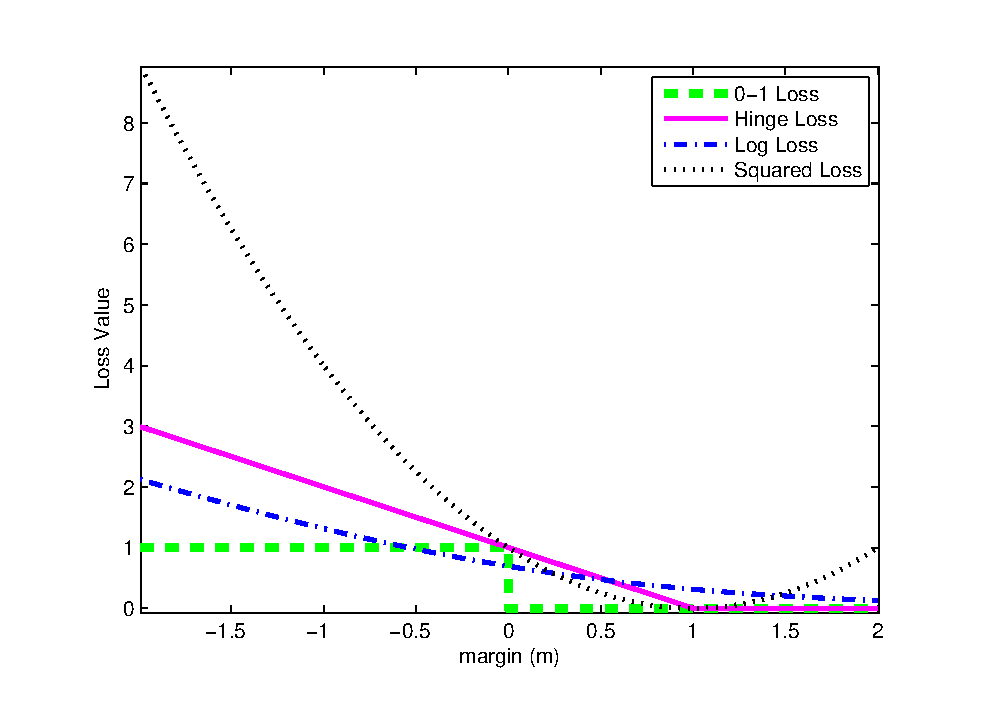
\includegraphics[width=0.50\textwidth]{images/fig13_losses.eps}
\vspace{-8mm}
\caption{ \footnotesize Different losses as a function of the margin.}
\label{fig:losses}
\end{figure}
%%%%%%%%%%%%%%%%%%%%%%%%%%%%%%%%%%%%%%%%%%%%%%%%%%%%%%%%%%%%%%%%%%%%

\MYCOMMENT

%%%%%%%%%%%%%%%%%%%%%%%%%%%%%%%%%%%%%%%%%%%%%%%%%%%%%%%%%%%%%%%%%%%%
\begin{figure}[t!]
\vspace{-3mm}
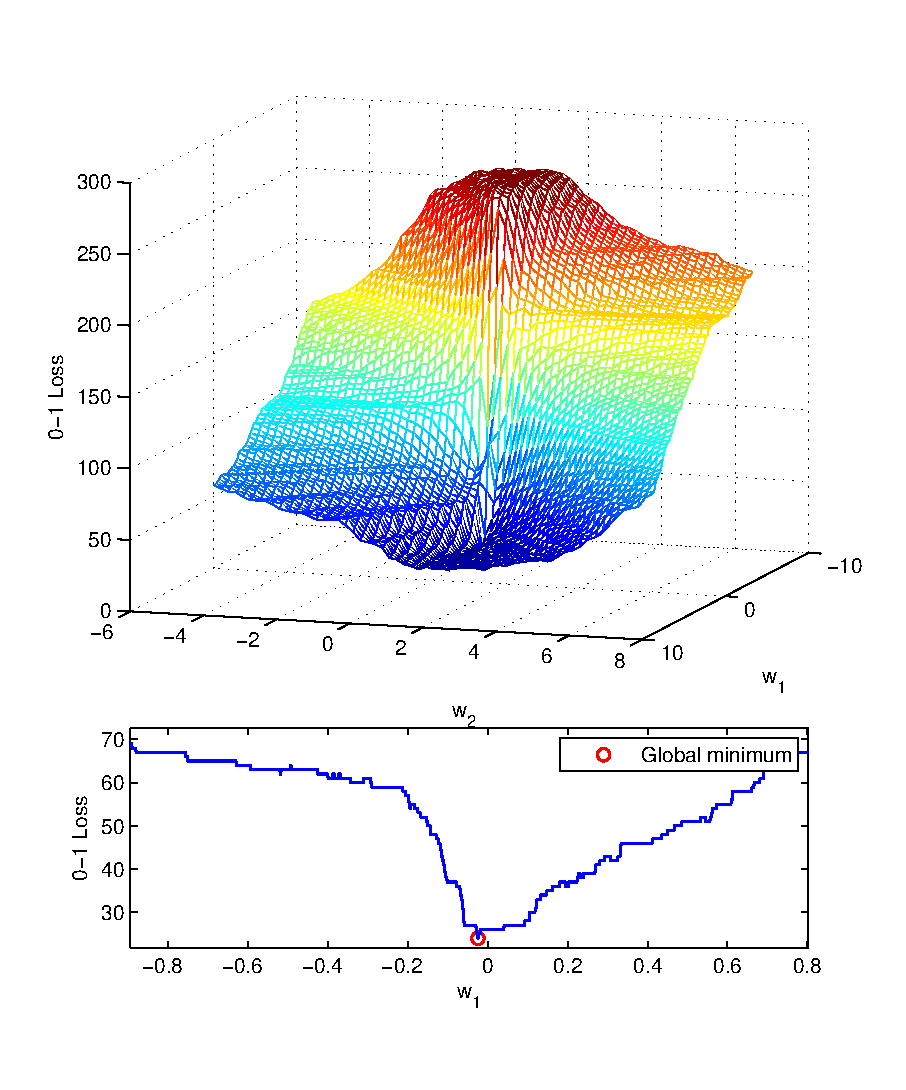
\includegraphics[width=0.50\textwidth]{images/fig14_complexshape.eps}
\vspace{-12mm}
\caption{ \footnotesize Complex shape of 0--1 loss.  The top
  figure plots 0--1 loss function of a two-dimensional dataset as a
  function of two varying weights $w_1$ and $w_2$. The bottom figure
  plots the same function with $w_2$ held fixed at its optimal
  value. 0--1 loss clearly has a non-smooth shape with numerous local
  optima, which get worse as dimensionality increases.}
\label{fig:complex_shape}
\end{figure}
%%%%%%%%%%%%%%%%%%%%%%%%%%%%%%%%%%%%%%%%%%%%%%%%%%%%%%%%%%%%%%%%%%%%

\ENDMYCOMMENT

We assume a $D$-dimensional data input vector $\x \in \R^D$ ($D$ for
dimension), where the goal of binary classification is to predict the
target class $\hat{t} \in \{ -1, 1 \}$ for a given $\x$.  Linear
binary classification which underlies many popular classification
approaches such as SVMs and logistic regression defines a predictor
function:
\begin{equation} 
\label{eq:predictor}
f_{\w}(\x) = \sum_{j=1}^D w_j x_j + w_0 = \w^T \x + w_0,
\end{equation}
where $w_j \in \mathbb{R}$ and $w_0 \in \mathbb{R}$ is a bias.  Then
\begin{equation}
\hat{t} = 
  \begin{cases}
  1  & f_{\w}(\x) \geq 0\\
  -1 & f_{\w}(\x) <    0
  \end{cases}
\end{equation}
Thus, the equation of the decision boundary that separates the two
classes is $f_{\w}(\x) = \w^T \x + w_0 = 0$, which is a
$D$-dimensional hyperplane.

We use two notations for the weight vector $\w$: in the
\emph{homogeneous} notation, we assume $\w = (w_0,w_1,\ldots,w_D)^T$
and $\x = (1,x_1,\ldots,x_D)$ so that $f_{\w}(\x) = \w^T \x$.  In the
\emph{non-homogeneous} notation, we assume $\w = (w_1,\ldots,w_D)^T$
and $\x = (x_1,\ldots,x_D)$ so that $f_{\w}(\x) = \w^T \x + w_0$.

The \emph{training dataset} contains $N$ data vectors $\X =
\{\x_1, \x_2, \dots, \x_N\}$ and their corresponding target
class $\t = \{t_1, t_2, \dots, t_N\}$. To measure the confidence of a
class prediction for an observation $\xi \in \X$, the so--called
\emph{margin} is defined as $m_i(\w) = t_i f_{\w}(x_i)$.  A margin
$m_i(\w) < 0$ indicates $\xi$ is misclassified, while $m_i(\w) \geq 0$
indicates $\xi$ is correctly classified and $m_i$ represents the
``margin of safety'' by which the prediction for $\xi$ is correct
\cite{McAllester}.

The learning objective in classification is to find the best
(homogenous) $\w$ to minimize some loss over the training data
$(\X,\t)$, i.e.,
\begin{equation}
\label{eq:objective}
 \w^* = \arg\min_{\w} \; \sum_{i=1}^{N} L(m_i(\w)) + \lambda R(\w),
\end{equation}
where loss $L(m_i(\w))$ is defined as a function of the margin for
each data point $\xi$, $R(\w)$ is a \emph{regularizer} which
prevents overfitting (typically $\|\w\|_2^2$ or $\|\w\|_1$), and
$\lambda > 0$ is the \emph{regularization strength parameter}.

Some popular losses as a function of the margin are
{\footnotesize
\begin{eqnarray}
\!\!\!\!\!\mbox{\bf 0--1 loss:} & \!\!\!\!\! L_{01}(m_i(\w))\!\!\!\!\! & = \mathbb{I} [m_i(\w) \leq 0], \label{eq:loss01} \\
\!\!\!\!\!\mbox{\bf squared loss:} & \!\!\!\!\! L_2(m_i(\w))\!\!\!\!\! &= \frac{1}{2}[m_i(\w) - 1]^2 \\
\!\!\!\!\!\mbox{\bf hinge loss:} & \!\!\!\!\! L_{hinge}(m_i(\w))\!\!\!\!\! &= \max(0, 1 - m_i(\w)) \\
\!\!\!\!\!\mbox{\bf log loss:} & \!\!\!\!\! L_{log}(m_i(\w))\!\!\!\!\! &= \ln (1 + e^{-m_i(\w)}) 
\end{eqnarray}}
where $\mathbb{I}[\cdot]$ is the indicator function taking the value 1
when its argument is true and 0 when false.  These losses are plotted
in Figure~\ref{fig:losses}.  0--1 loss is robust to outliers since it
is not affected by a misclassified point's distance from the margin,
but this property also makes it non-convex; the convex squared, hinge,
and log losses are not robust to outliers in this way since their
penalty does scale with the margin of misclassification.  Squared loss is
not an ideal loss for classification since it harshly penalizes a
classifier for correct margin predictions $\gg 1$, unlike the other
losses.  This leaves us with hinge loss as optimized in the SVM and
log loss as optimized in logistic regression as two convex surrogates
of 0--1 loss for later empirical comparison.

%%%%%%%%%%%%%%%%%%%%%%%%%%%%%%%%%%%%%%%%%%%%%%%%%%%%%%%%%%%%%%%%%%%%
%%%%%%%%%%%%%%%%%%%%%%%%%%%%%%%%%%%%%%%%%%%%%%%%%%%%%%%%%%%%%%%%%%%%
%%%%%%%%%%%%%%%%%%%%%%%%%%%%%%%%%%%%%%%%%%%%%%%%%%%%%%%%%%%%%%%%%%%%

\MYCOMMENT

{\bf 0--1 Loss:} 
\begin{equation}
L_{01}(m) = \left\{
     \begin{array}{ll}
       0 & : \text{if }m > 0\\
       1 & : \text{otherwise}
     \end{array}
   \right.
   \; = \; \mathbb{I} [m \leq 0], \label{eq:loss01}
\end{equation}
where the indicator function, $\mathbb{I} [.]$, is used to simplify
the piecewise function. In the context of linear binary classification
given in previous subsection, the margin is given by Equation
\ref{eq:margin}, and the objective given by Equation
\ref{eq:objective}.

{\bf Squared Loss:}
\begin{align}
L_2(m_i(\w)) &= \frac{1}{2}[m_i(\w) - 1]^2 = \frac{1}{2}[t_i f_{\w}(\xi) - t_i^2]^2 = \frac{1}{2}t_i^2 [f_{\w}(\xi) - t_i]^2 \nonumber \\
& = \frac{1}{2}[\w^T\xi - t_i]^2 \label{eq:loss2}
\end{align}
where we used the fact that $t_i^2 = 1$, and the constant
$\frac{1}{2}$ is used for later convenience. We see that minimizing
(the sum of) squared loss is equivalent to minimizing the (total
squared) difference between the value given by the predictor function
$\w^T\xi$ and the training target $t_i$.

{\bf Hinge Loss (SVM):}

The hinge loss is defined as
\[ \begin{split}
L_{hinge}(m_i(\w)) &= \max(0, 1 - m_i(\w)) \\
&= \max(0, 1 - t_i \w^T \xi),
\end{split} \] 
and it can be viewed as a piecewise linear approximation of log loss,
because it has the same properties as given for log loss for cases
when $m_i >> 1$ and $m_i << -1$.

{\bf Log Loss (Logistic Regression):}

We have discussed in Subsection \ref{ssec:binclass}, that if $m_i < 0$
then $|m_i|$ is a measure of the margin by which the class prediction
for $\xi$ given by $f_{\w}(x_i)$ is wrong, otherwise the prediction is
correct. In this sense, the log loss is defined as
\[ \begin{split}
L_{log}(m_i(\w)) &= \ln (1 + e^{-m_i(\w)}) \\
 &= \ln (1 + e^{-t_i\w^T\xi}) 
\end{split} \] 
It can be easily verified, that this loss is convex, and for $m_i >>
1$ we have $L_{log}(m_i) \approx 0$, on the other hand, for $m_i <<
-1$ we have $L_{log} \approx -m_i = |m_i|$. In other words, log loss
is a convex model of the scheme, where misclassification is penalized
by the absolute value of the margin, and correct classification has
zero penalty. We note that both log loss and quadratic loss can be
viewed as an attempt to estimate $P(t|\x)$ and can be derived under
assumption that $P(\x|t)$ has (multivariate) Gaussian distribution.

\ENDMYCOMMENT

%%%%%%%%%%%%%%%%%%%%%%%%%%%%%%%%%%%%%%%%%%%%%%%%%%%%%%%%%%%%%%%%%%%%
%%%%%%%%%%%%%%%%%%%%%%%%%%%%%%%%%%%%%%%%%%%%%%%%%%%%%%%%%%%%%%%%%%%%
%%%%%%%%%%%%%%%%%%%%%%%%%%%%%%%%%%%%%%%%%%%%%%%%%%%%%%%%%%%%%%%%%%%%

\MYCOMMENT

\subsubsection{Bayes Point Machine}

Bayes point machine (BPM) was proposed by \cite{Herbrich}. This is a
Bayesian approach to linear classification and is briefly summarized
as follows. From our discussion in Subsection \ref{ssec:binclass} we
see that, in linear classification, a point $\x$ is classified by $t =
\sign(\w^T \x)$ for some weight vector $\w$. Given the training
dataset $\D = \{\X, \t \}$, the likelihood for $\w$ is given by
$$p(\D | \w) = \prod_{i=1}^N p(t_i | \xi, \w) = \prod_{i=1}^N
\phi(\frac{t_i\w^T\xi}{\epsilon}),$$ where
$$\phi(z) = \int_{-\infty}^z N(z; 0, 1) dz,$$ and $\epsilon$ controls
the allowed `slack'. By using $\phi$ instead of a step function, this
likelihood tolerates small errors. Under the Bayesian approach, we
also have a prior distribution of $\w$, which is taken to be the
zero-mean unit-variance normal distribution: $N(\boldsymbol{0,
  I})$. Given this model, the optimal way to classify a new data point
$\x$ is to vote all classifiers according to their posterior
probability: $\mathbb{E}[\sign(\w^T \x) | \D]$. This is, however,
expensive to compute. As an approximation to this, BPM uses the output
of the average classifier: $\sign(\mathbb{E}[\w] ^T \x)$. This can be
estimated by the billiard ball algorithm proposed in the original BPM
paper, which is based on the Monte Carlo method. Another (better) way
to estimate this is by using expectation propagation as proposed by
\cite{bpm}. This thesis uses the Matlab implementation of expectation
propagation algorithm for BPM of the latter author in all comparisons
where BPM is present.

\subsubsection{Other Methods}

Apart from mentioned algorithms, there are quite a few other
algorithms that can solve the binary classification problem. Some of
the most notable are, for example, the following. Neural networks
\cite{bishop2} consist of one or more interconnected layers of
neurons, each neuron having its own weight vector. It can be viewed as
an adaptive system that changes its structure during learning
phase. In contrast to the introduced linear binary classification
model, neural networks is generally not linear, except for perceptrons
\cite{perceptron}, which can be considered as the simplest kind of
neural network. Perceptron, however, may not converge if the two
classes are not linearly separable. $k-$ Nearest Neighbor \cite{kNN}
is one of the simplest classification algorithms. It assigns a new
data point to the class most common amongst its $k$ nearest training
data points (neighbors). Adaboost \cite{adaboost}, short for Adaptive
Boosting, is an algorithm that coordinate several weak classifiers to
improve the classification quality, where subsequent classifiers are
tweaked in favor of those instances misclassified by previous
classifiers. Adaboost uses exponential loss, which is $L_{exp} =
\exp(-m_i(\w)) = \exp(-t_i\w^T\xi)$, hence can be sensitive to noisy
data and outliers. Decision trees are also used for classification as
shown by \cite{tree1}, and by \cite{tree2}.

There are also many works that are more or less related to the work of
this thesis. We can categorize them into those developing classifiers
that are robust to outliers and those optimizing 0--1 loss
directly. The number of works in the first category is quite abundant,
including t-logistic regression \cite{Ding}, robust truncated hinge
loss \cite{robusthinge}, SavageBoost \cite{lossdesign}, and
more. There are, however, almost no works in the second category. At
the time of finishing this thesis, we can only find the work by
\cite{ling}, which proposes an algorithm optimizing 0--1 loss for
perceptrons by random coordinate descent.

\ENDMYCOMMENT
